\documentclass[10pt,dvipsnames]{beamer}

\definecolor{links}{HTML}{2A1B81}
\hypersetup{colorlinks,linkcolor=,urlcolor=links}

\usetheme{metropolis}
\metroset{block=fill}
\setmonofont{Ubuntu Mono}

\usepackage{appendixnumberbeamer}

\usepackage{booktabs,empheq,bbold,bm}
\usepackage[scale=2]{ccicons}

\usepackage{pgfplots}
\usepgfplotslibrary{dateplot}

\usepackage{xspace}
\newcommand{\themename}{\textbf{\textsc{metropolis}}\xspace}

% for python listings; inspired by https://gist.github.com/YidongQIN/a10dd4f72381362aff4257e7a5541d86 
\usepackage{listings}
\usepackage{color}
\definecolor{darkred}{rgb}{0.6,0.0,0.0}
\definecolor{darkgreen}{rgb}{0,0.50,0}
\definecolor{lightblue}{rgb}{0.0,0.42,0.91}
\definecolor{orange}{rgb}{0.99,0.48,0.13}
\definecolor{grass}{rgb}{0.18,0.80,0.18}
\definecolor{pink}{rgb}{0.97,0.15,0.45}
\lstdefinelanguage{PythonPlus}[]{Python}{
  morekeywords=[1]{,as,assert,nonlocal,with,yield,self,True,False,None,} % Python builtin
  morekeywords=[2]{,__init__,__add__,__mul__,__div__,__sub__,__call__,__getitem__,__setitem__,__eq__,__ne__,__nonzero__,__rmul__,__radd__,__repr__,__str__,__get__,__truediv__,__pow__,__name__,__future__,__all__,}, % magic methods
  morekeywords=[3]{,object,type,isinstance,copy,deepcopy,zip,enumerate,reversed,list,set,len,dict,tuple,range,xrange,append,execfile,real,imag,reduce,str,repr,}, % common functions
  morekeywords=[4]{,Exception,NameError,IndexError,SyntaxError,TypeError,ValueError,OverflowError,ZeroDivisionError,}, % errors
  morekeywords=[5]{,ode,fsolve,sqrt,exp,sin,cos,arctan,arctan2,arccos,pi, array,norm,solve,dot,arange,isscalar,max,sum,flatten,shape,reshape,find,any,all,abs,plot,linspace,legend,quad,polyval,polyfit,hstack,concatenate,vstack,column_stack,empty,zeros,ones,rand,vander,grid,pcolor,eig,eigs,eigvals,svd,qr,tan,det,logspace,roll,min,mean,cumsum,cumprod,diff,vectorize,lstsq,cla,eye,xlabel,ylabel,squeeze,}, % numpy / math
}
\lstdefinestyle{colorEX}{
  basicstyle=\ttfamily\small,
  backgroundcolor=\color{white},
  commentstyle=\color{darkgreen}\slshape,
  keywordstyle=\color{blue}\bfseries\itshape,
  keywordstyle=[2]\color{blue}\bfseries,
  keywordstyle=[3]\color{grass},
  keywordstyle=[4]\color{red},
  keywordstyle=[5]\color{orange},
  stringstyle=\color{darkred},
  emphstyle=\color{pink}\underbar,
}
\lstset{style=colorEX,
        basewidth = {.49em}}

\newcommand{\bn}{\mathbf{n}}
\newcommand{\bq}{\mathbf{q}}
\newcommand{\bu}{\mathbf{u}}

\newcommand{\hbn}{\hat{\mathbf{n}}}
\newcommand{\hbx}{\hat{\mathbf{x}}}
\newcommand{\hbz}{\hat{\mathbf{z}}}

\newcommand{\bU}{\mathbf{U}}

\newcommand{\bpsi}{\bm{\psi}}
\newcommand{\bzero}{\bm{0}}

\newcommand{\eps}{\epsilon}
\newcommand{\grad}{\nabla}
\newcommand{\Div}{\nabla\cdot}

\newcommand{\rhoi}{\rho_{\text{i}}}
\newcommand{\snew}{s^{\text{new}}}

\newcommand{\comm}[1]{{\footnotesize \hfill \emph{#1}}}

\title{numerical modeling of glaciers}
%\subtitle{version 1.0}
\date{June 2024}
\author{Ed Bueler}
\institute{Porphyry Place, McCarthy, Alaska \\ \phantom{foo} \\ version 1.0}
\titlegraphic{\vspace{-1cm}\par\hspace{-1cm}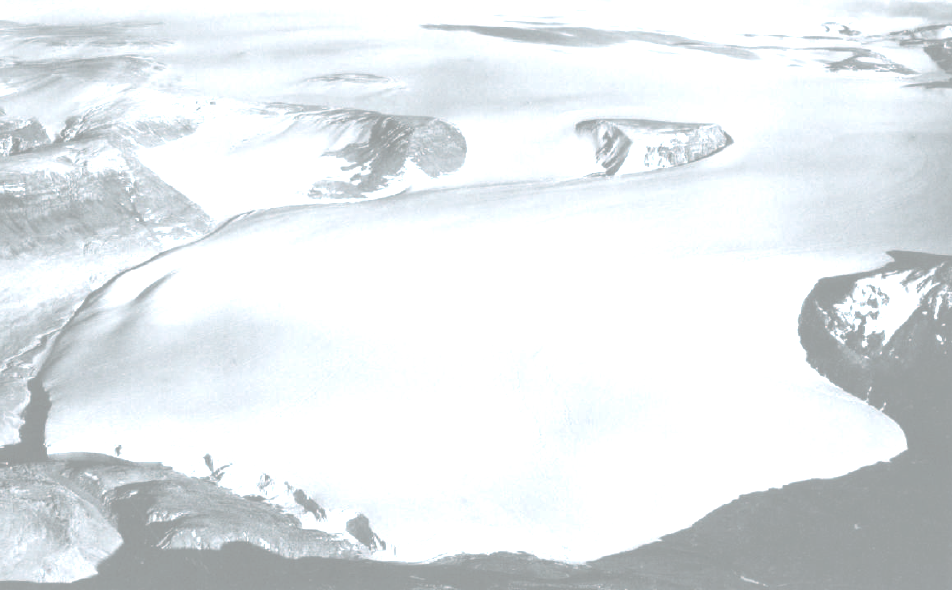
\includegraphics[width=1.5\textwidth]{polaris-overexposed.png}}

\begin{document}
\graphicspath{{figs/}{../figures/}}

\maketitle

\begin{frame}{Outline}
  %\setbeamertemplate{section in toc}[sections numbered]
  %\tableofcontents[hideallsubsections]
  \tableofcontents
\end{frame}


\begin{frame}{online materials}

\begin{itemize}
\item these are my \alert{new slides} \dots\xspace please let me know how it works?
\item in any case, \alert{please ask questions at any time!}
\end{itemize}

\bigskip

\metroset{block=fill}
\begin{block}{online materials}

my slides, notes, codes, and materials are hosted at

\medskip
\centerline{\href{https://github.com/bueler/mccarthy}{\texttt{github.com/bueler/mccarthy}}}
\end{block}

\medskip
{\footnotesize
these slides: \href{https://github.com/bueler/mccarthy/blob/master/slides/slides-2024.pdf}{\texttt{slides/slides-2024.pdf}}

exercises: \href{https://github.com/bueler/mccarthy/blob/master/slides/exercises-2024.pdf}{\texttt{slides/exercises-2024.pdf}}

notes: \href{https://github.com/bueler/mccarthy/blob/master/notes/notes-2024.pdf}{\texttt{notes/notes-2024.pdf}}

Python codes: \href{https://github.com/bueler/mccarthy/tree/master/py}{\texttt{py/}}

project 13,14 Python codes: \href{https://github.com/bueler/mccarthy/tree/master/stokes}{\texttt{stokes/}}

}
\end{frame}


\section[how does the surface of a glacier move?]{\textbf{how does the surface of a glacier move?} (hour 1)}

\subsection{basic mathematics}


\begin{frame}{surface motion}

\bigskip
\begin{center}
\includegraphics<1>[width=\textwidth]{noboat}
%\includegraphics<2>[width=\textwidth]{boat}
%\includegraphics<3>[width=\textwidth]{boatplus}
\includegraphics<2>[width=\textwidth]{boatplus}
\end{center}


%LIVE really the question is, "what is the most basic thing you can say mathematically at the surface of a glacier?"
%LIVE imagine a magic glacier boat which always floats on the top of the ice.
\end{frame}

\begin{frame}{surface motion: notation}
\begin{center}
\begin{tikzpicture}[scale=1.2]
\node[inner sep=0pt] (domain) at (0,0)
    {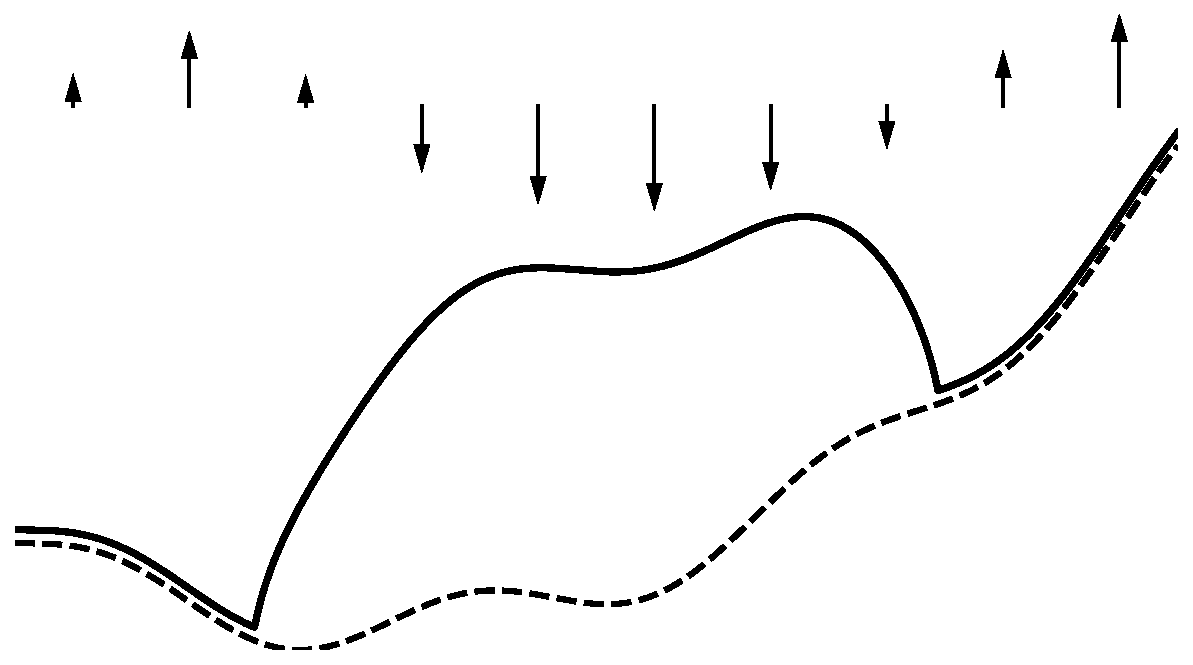
\includegraphics[width=0.72\textwidth]{domain}};
\node (a) at (-2.5,0.8) {$a(t,x)$};
\node (b) at (1.5,-1.0) {$b(x)$};
\node (s) at (-1.6,0.0) {$s(t,x)$};
\node (u) at (0.0,-0.5) {$\bu(t,x,z)$};
\end{tikzpicture}
\end{center}

\vspace{-3mm}
\begin{itemize}
\item two spatial dimensions $x,z$ \comm{\dots\, at least for a while}
\item $z = b(x)$: bed elevation (m) \comm{fixed}
\item $z = s(t,x)$: ice surface elevation (m)
\item $\bu(t,x,z)=(u,w)$: ice velocity ($\text{m}\,\text{s}^{-1}$)
\item $a(t,x)$: surface mass balance in ice-equivalent units ($\text{m}\,\text{s}^{-1}$)
%\item {\color{NavyBlue} $z = s(t,x)$}: ice surface elevation (m)
%\item {\color{NavyBlue} $\bu(t,x,z)=(u,w)$}: ice velocity ($\text{m}\,\text{s}^{-1}$)
%\item {\color{Orange} $a(t,x)$}: surface mass balance in ice-equivalent units ($\text{m}\,\text{s}^{-1}$)
\end{itemize}
\end{frame}


\begin{frame}{surface kinematical equation (SKE)}
\begin{center}
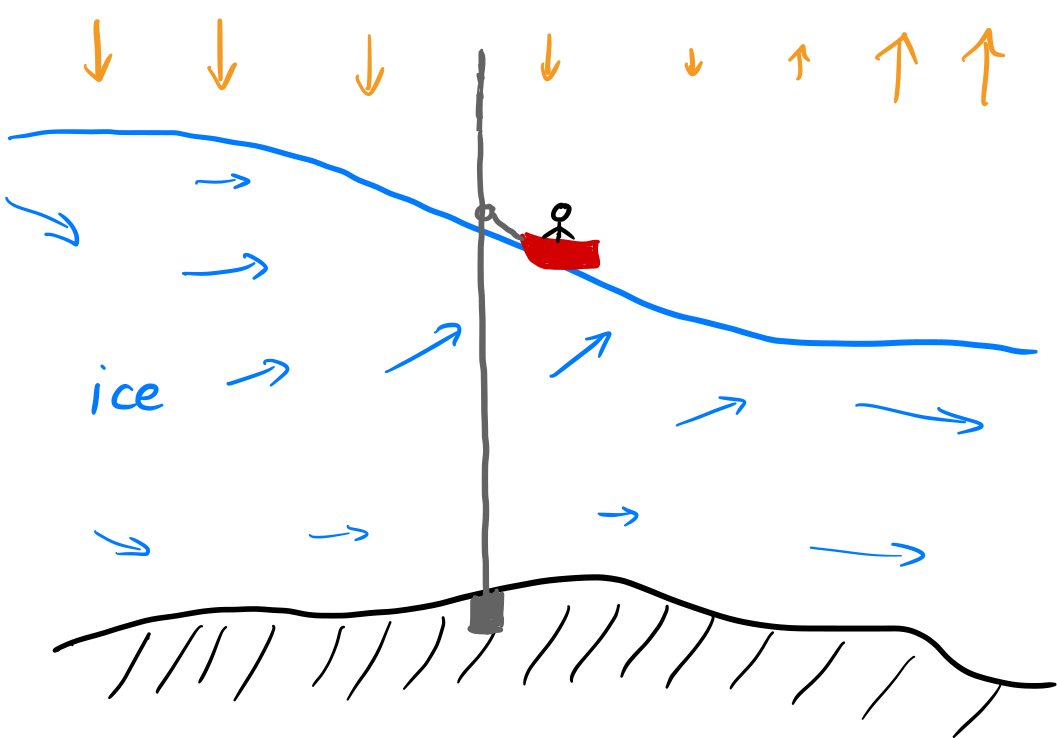
\includegraphics[width=0.5\textwidth]{boatplus}
\end{center}

\vspace{-5mm}
\begin{equation*}
\frac{\partial s}{\partial t} = \uncover<2-4>{a} \uncover<3-4>{+w} \uncover<4>{-u \frac{\partial s}{\partial x}}
\end{equation*}

the ice surface moves up and down according to
\begin{itemize}
\item<2-4> surface mass balance (SMB) \comm{(\emph{climatic} mass balance ice equiv.)}
\item<3-4> vertical component of ice velocity
\item<4> horizontal component of ice velocity \emph{and surface slope}
\end{itemize}
\end{frame}

\begin{frame}{surface kinematical equation (SKE) \dots alternate form}
\begin{center}
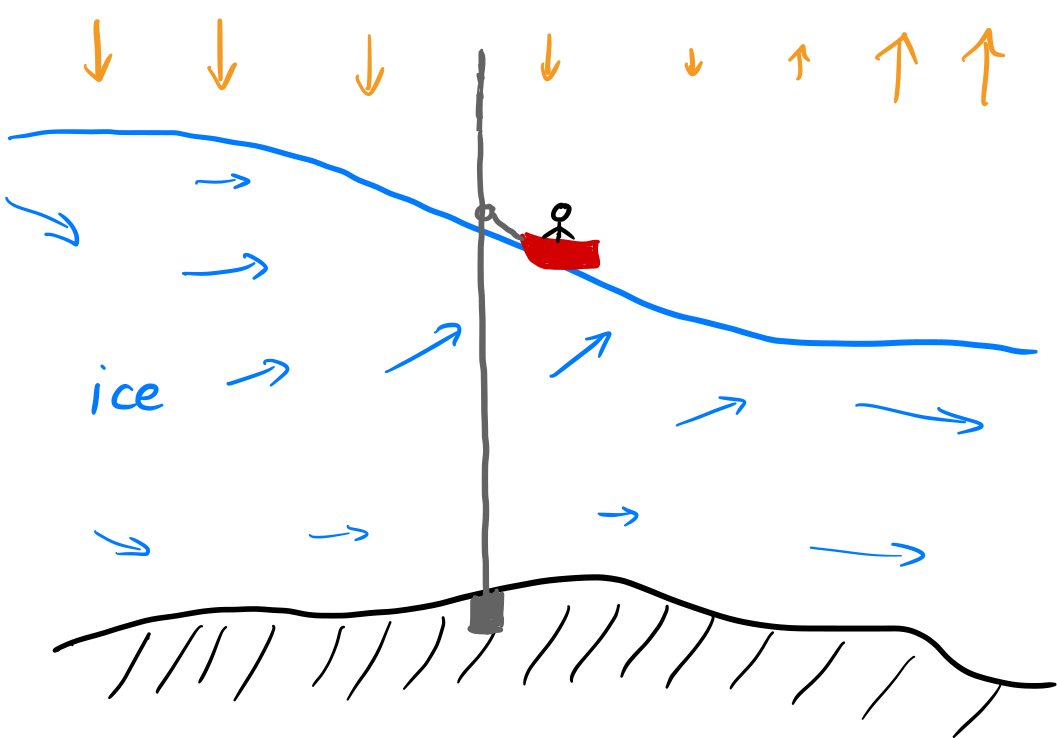
\includegraphics[width=0.5\textwidth]{boatplus}
\end{center}

\vspace{-5mm}
\begin{equation*}
\frac{\partial s}{\partial t} = a + \bu \cdot \bn_s
\end{equation*}

\begin{itemize}
\item $\bn_s$ is a vector which points upward and is normal (perpendicular) to the ice surface:
	$$\bn_s = \left(-\frac{\partial s}{\partial x}, \,1\right)$$
\item recall: $\bu=(u,w)$
\end{itemize}
\end{frame}


\begin{frame}{plan for hour 1: SKE as a numerical glacier geometry model}

\begin{itemize}
\item \alert{model:} the planar surface kinematical equation (SKE)
\begin{equation*}
\frac{\partial s}{\partial t} - \bu \cdot \bn_s = a \qquad \iff \qquad \frac{\partial s}{\partial t} + u \frac{\partial s}{\partial x} = a + w
\end{equation*}

    \begin{itemize}
    \item[$\circ$] assume $a,u,w$ are given functions/values \uncover<2>{\hfill \alert{$\leftarrow$ this needs fixing!}}
    \end{itemize}
\item \alert{numerical modeling goal:} use a computer program to evolve the glacier surface $z=s(t,x)$
    \begin{itemize}
    \item[$\circ$] one short Python program in 1D: \quad \href{https://github.com/bueler/mccarthy/blob/master/py/surface1d.py}{py/surface1d.py}
    \end{itemize}
\item \alert{to address:}
     \begin{enumerate}
     \item how to compute time-dependent solutions?
     \item accuracy and stability?
     \item how to compute steady state solutions?
     \item practical: debugging, verification, visualization?
     \end{enumerate}
\end{itemize}
\end{frame}


\begin{frame}[standout]
claim: the central object of glacier theory

is the surface kinematical equation

\begin{equation*}
\frac{\partial s}{\partial t} + u \frac{\partial s}{\partial x} = a + w
\end{equation*}
\end{frame}


\begin{frame}{surface smoothness versus thickness smoothness}

\bigskip
\begin{center}
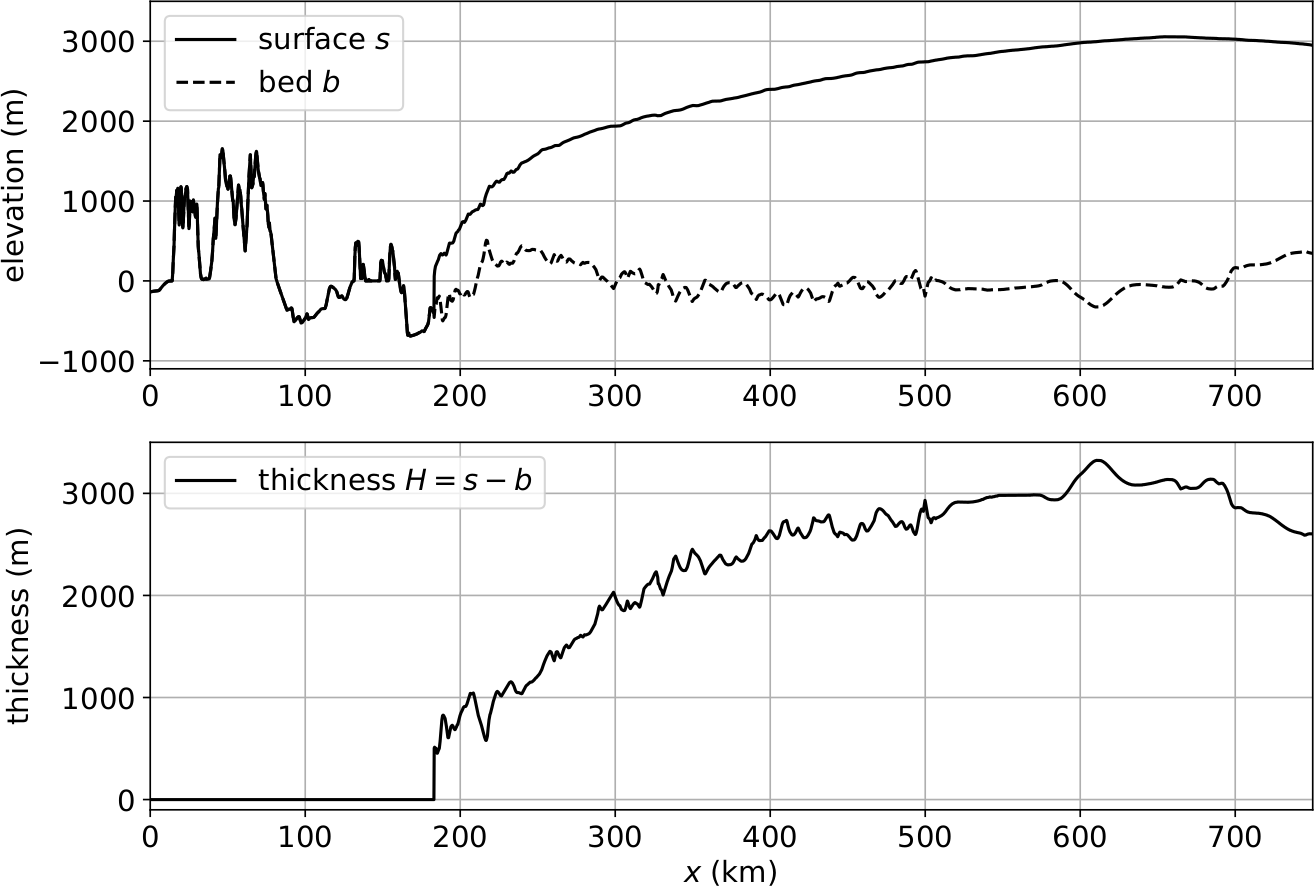
\includegraphics[width=0.95\textwidth]{giscross}
\end{center}

\hfill \tiny [Data from Morlighem et al (2017), and thanks to A.~Aschwanden]
\end{frame}


\subsection{some numerics}


\begin{frame}{discretize the SKE 1}

\begin{center}
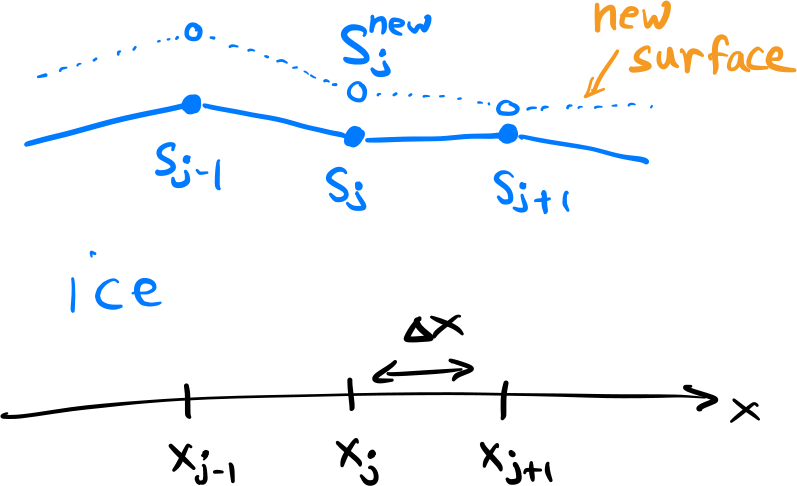
\includegraphics[width=0.7\textwidth]{surfacenotation}
\end{center}
\end{frame}


\begin{frame}{discretize the SKE 2}
\begin{center}
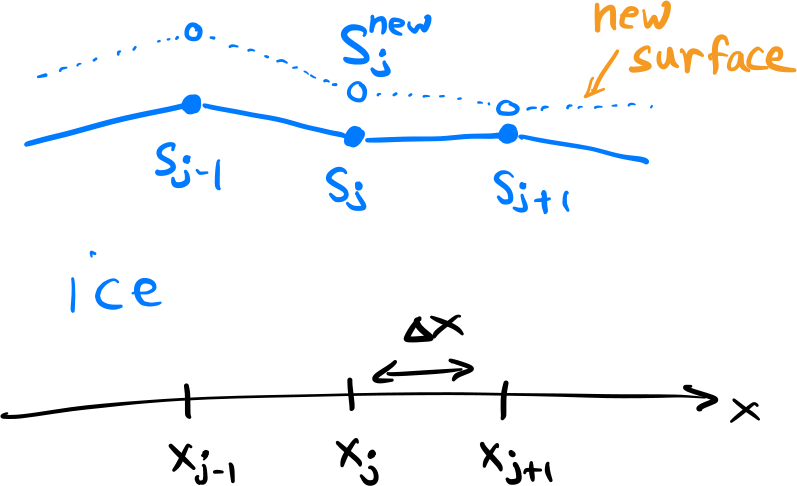
\includegraphics[width=0.5\textwidth]{surfacenotation}
\end{center}

\begin{itemize}
\item SKE: $\displaystyle \frac{\partial s}{\partial t} + u \frac{\partial s}{\partial x} = a + w$

\smallskip
\item choose time step $\Delta t>0$ and grid spacing $\Delta x>0$
\item approximate partial derivatives by finite difference\footnote{helpful textbooks include LeVeque \cite{Leveque2007} and Morton \& Mayers \cite{MortonMayers2005}} quotients:
    $$\frac{\partial s}{\partial t} \approx \frac{\snew_j - s_j}{\Delta t}, \qquad \frac{\partial s}{\partial x} \approx \frac{s_{j+1} - s_{j-1}}{2\Delta x}$$
\phantom{foo}
\end{itemize}
\end{frame}


\begin{frame}{discretize the SKE 3}
\begin{center}
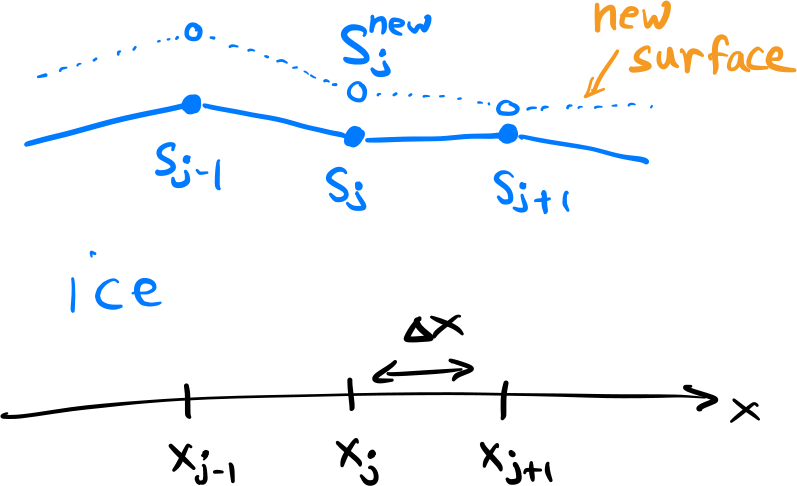
\includegraphics[width=0.5\textwidth]{surfacenotation}
\end{center}

\begin{itemize}
\item now SKE\, $\left(\frac{\partial s}{\partial t} + u \frac{\partial s}{\partial x} = a + w\right)$\, becomes a discrete equation:
    $$\frac{\snew_j - s_j}{\Delta t} + u_j \frac{s_{j+1} - s_{j-1}}{2\Delta x} = a_j + w_j$$
\item which we can write as an update which determines $\snew_j$:
	$$\snew_j = s_j - \Delta t\, u_j \frac{s_{j+1}-s_{j-1}}{2\Delta x} + \Delta t (a_j + w_j)$$
\end{itemize}
\end{frame}


\begin{frame}{upwinding}

\begin{itemize}
\item \alert{however \dots}
\item if we implement this ``forward-time centered-space'' scheme
	$$\snew_j = s_j - \Delta t\, u_j \frac{s_{j+1}-s_{j-1}}{2\Delta x} + \Delta t (a_j + w_j) \hspace{1.0cm} \leftarrow \text{\emph{\alert{bad}}}$$
then bad things happen! \comm{exercise?}
\item instead, it is known that when the ``advecting velocity'' is positive ($u_j \ge 0$) then the ``upwind'' version is conditionally stable:
	$$\hspace{3mm} \snew_j = s_j - \Delta t\, u_j \frac{s_j-s_{j-1}}{\Delta x} + \Delta t (a_j + w_j) \hfill \hspace{1.2cm} \leftarrow \text{\emph{useful}}$$

    \begin{itemize}
    \item[$\circ$] upwind formula: \quad $\displaystyle \frac{\partial s}{\partial x} \approx \frac{1}{\Delta x} \begin{cases} (s_j-s_{j-1}), & u_j \ge 0 \\ (s_{j+1}-s_j), & u_j < 0 \end{cases}$
    \item[$\circ$] the condition for stability is known \comm{demo soon}
    \end{itemize}
%\item see textbooks for these caveats
\end{itemize}
\end{frame}


\begin{frame}[fragile]\frametitle{implementation}

\begin{itemize}
\item this upwind scheme for the SKE (assumes $u_j \ge 0$):
    $$\snew_j = s_j - \Delta t\, u_j \frac{s_j-s_{j-1}}{\Delta x} + \Delta t (a_j + w_j)$$
becomes a Python function:
\end{itemize}
\begin{lstlisting}[language=PythonPlus]
def explicitstep(s, x, dt):
    dx = x[1] - x[0]
    snew = s.copy()
    snew[1:] -= dt * u(x[1:]) * (s[1:] - s[:-1]) / dx  # assumes u >= 0
    snew[1:] += dt * (a(x[1:]) + w(x[1:]))
    return snew
\end{lstlisting}

\vspace{-2mm}
{\footnotesize
    \begin{itemize}
    \item[$\circ$] \texttt{x}, \texttt{s}, \texttt{snew} are 1D NumPy arrays
    \item[$\circ$] separate functions define $a(x)$, $u(x)$, $w(x)$ \comm{(need to make up some values?)}
    \item[$\circ$] \texttt{x} is equally-spaced
    \item[$\circ$] $j=$\texttt{[1:]} indicates all indices except zero
    \item[$\circ$] note that \, \texttt{snew[0] = s[0]} \, is never changed; this is a boundary condition
    \end{itemize}
}
\end{frame}


\begin{frame}[fragile]
\frametitle{live demo: evolution of glacier surface}
\begin{center}
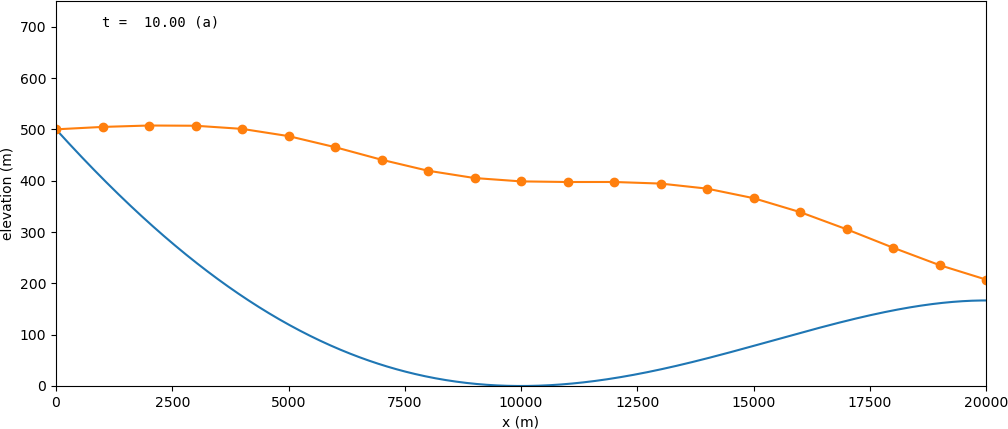
\includegraphics[width=0.7\textwidth]{frame010}
\end{center}

\bigskip
\begin{block}{live demo}
\begin{itemize}
\item run \href{https://github.com/bueler/mccarthy/blob/master/py/surface1d.py}{py/surface1d.py}:
\begin{verbatim}
$ python3 surface1d.py
$ eog output/frame*.png          # any image viewer
\end{verbatim}
\item the following example modifications reveal stability issues:
    \begin{enumerate}
    \item increase velocity: \quad $u(x)$ \, $\to$ \, $2.5\, u(x)$
    \item increase resolution: \quad $\Delta x=1000$ m \, $\to$ \, $\Delta x=400$ m
    \item lengthen time-steps: \quad $\Delta t = 1$ a \, $\to$ \, $\Delta t = 2.5$ a
    \end{enumerate}
\end{itemize}
\end{block}
\end{frame}


\begin{frame}{condition for time-stepping stability}

\bigskip\medskip
\begin{itemize}
\item if horizontal velocity $u$ is given

in the SKE $\left(\frac{\partial s}{\partial t} + u \frac{\partial s}{\partial x} = a + w\right)$,

then info about the surface

travels at speed $u$
\item from this $(t,x)$ grid picture, the

upwind scheme can only be

stable if
$$|u_j| \Delta t \le \Delta x \hspace{40mm}$$

for every $j$
    \begin{itemize}
    \item[$\circ$] observed by Courant, Friedrichs, and Lewy (1928)
    \end{itemize}

\vspace{-45mm}
\hfill 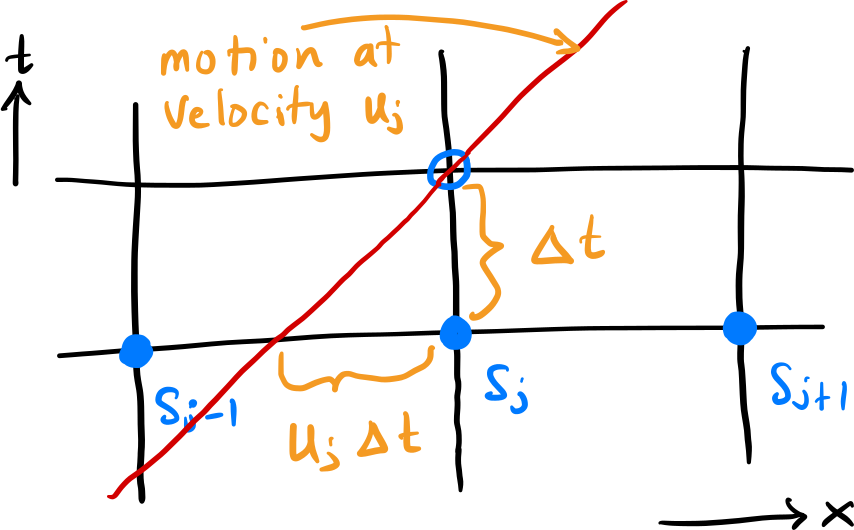
\includegraphics[width=0.43\textwidth]{cfl.png}

\vspace{15mm}
\item rearranged, this is the \alert{CFL condition} on the time step:
$$\Delta t \le \frac{\Delta x}{\max |u_j|} \hspace{40mm}$$
\end{itemize}
\end{frame}


\begin{frame}[fragile]
\frametitle{live demo: steady state of a glacier surface}
\begin{center}
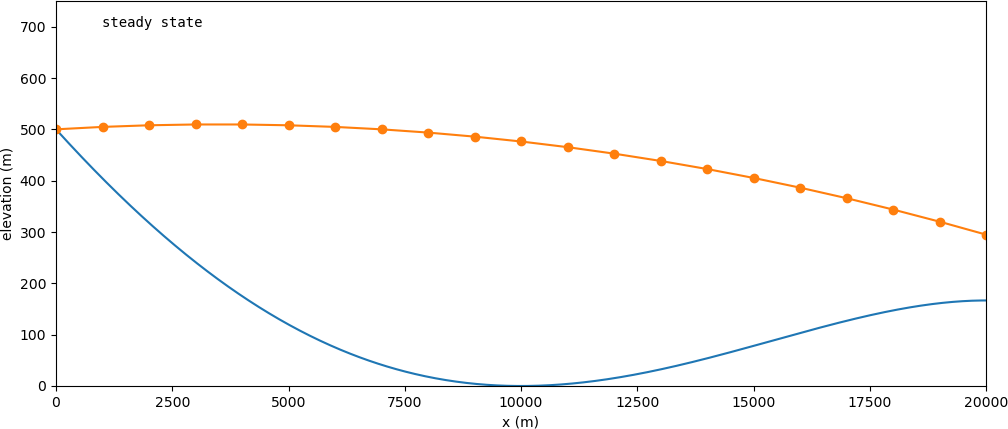
\includegraphics[width=0.7\textwidth]{steady}
\end{center}

\bigskip
\begin{itemize}
\item SKE in steady-state ($\frac{\partial s}{\partial t}=0$): \quad $\displaystyle u \frac{\partial s}{\partial x} = a + w$
\end{itemize}

\begin{block}{live demo}
\begin{itemize}
\item same run as before, but view steady-state output:
\begin{verbatim}
$ eog output/steady.png
\end{verbatim}
\item the following modification reveals an issue:
    \begin{enumerate}
    \item double SMB: \quad $a(x)$ \, $\to$ \, $2 a(x)$
    \end{enumerate}
\end{itemize}
\end{block}
\end{frame}


\begin{frame}{teaser: 2D steady state of a glacier surface}

\begin{itemize}
\item this example uses \href{https://www.firedrakeproject.org/}{Firedrake}
{\footnotesize
    \begin{itemize}
    \item[$\circ$] \emph{talk to me?}
    \item[$\circ$] \emph{or project 6, 13, 14 people!}
    \end{itemize}
}
\item code: \href{https://github.com/bueler/mccarthy/blob/master/py/surface2d.py}{py/surface2d.py}

\item result: $\rightarrow$

\vspace{-25mm}
\mbox{\hspace{60mm} 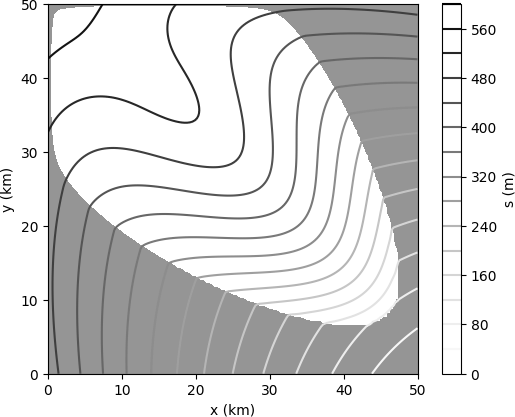
\includegraphics[width=0.45\textwidth]{surface2d}}

\vspace{-12mm}
\item solves 2D steady-state SKE:
\begin{align*}
&& u \frac{\partial s}{\partial x} + v \frac{\partial s}{\partial y} &= a + w \hspace{40mm}\\
\text{\emph{or}} && (u,v) \cdot \grad s &= a + w \\
\text{\emph{or}} && -\bu \cdot \bn_s &= a
\end{align*}

{\footnotesize
    \begin{itemize}
    \item[$\circ$] where $\bn_s = (-\frac{\partial s}{\partial x},-\frac{\partial s}{\partial y},1) = (-\grad s,1)$
    \end{itemize}
}

\smallskip
\item \alert{but subject to $s \ge b$}

\medskip
\item compare time-dependent SKE in 2D: \quad $\displaystyle \frac{\partial s}{\partial t} - \bu \cdot \bn_s = a$
\end{itemize}
\end{frame}


\begin{frame}[standout]
let's talk about all the (many) issues

when numerically solving the SKE

\vspace{10mm}
\begin{center}
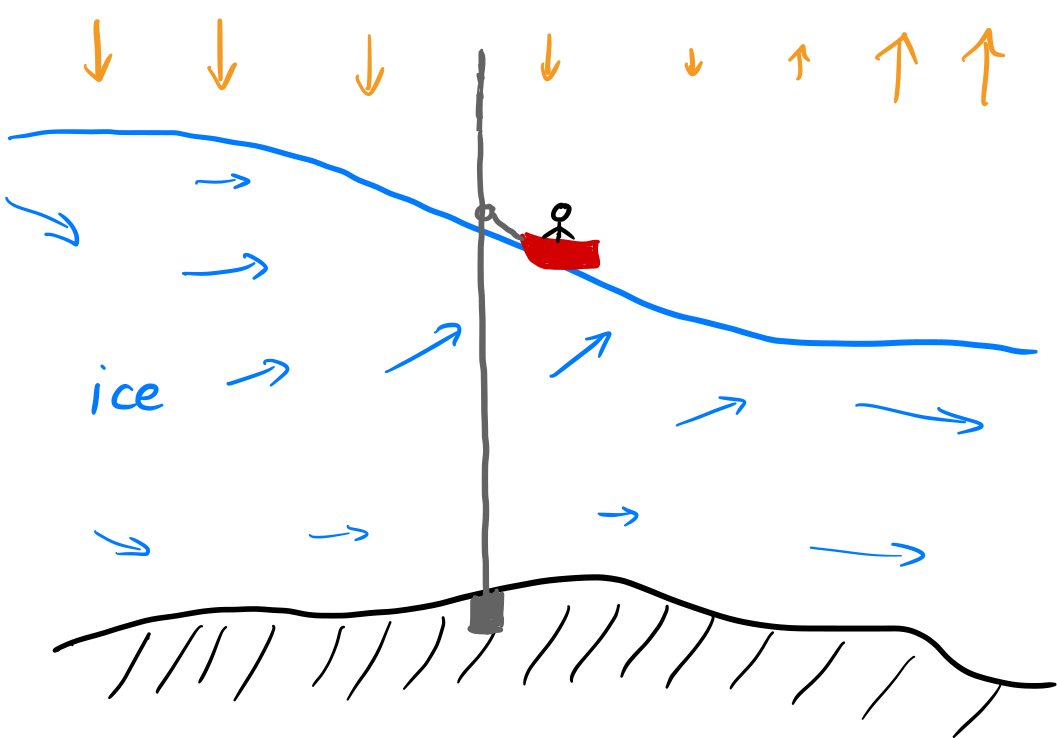
\includegraphics[width=0.5\textwidth]{boatplus}
\end{center}
\end{frame}


\begin{frame}{many issues}
\begin{itemize}
\item[] \alert{MAJOR modeling issues}
    \begin{enumerate}
    \item whence the SMB $a$? \comm{Regine!}
    \item whence the surface velocity $u,w$? \comm{2nd hour!}
    \end{enumerate}
\item[] \alert{mathematical issues}
    \begin{enumerate}\setcounter{enumi}{2}
    \item is the time-dependent SKE well-posed for (various) given-field, initial condition, \& boundary condition assumptions?
    \item is the steady-state SKE well-posed for (various) \dots \, assumptions?
    \item how do we understand admissibility $s\ge b$ in the theory?
    \end{enumerate}
\item[] \alert{numerical issues}
    \begin{enumerate}\setcounter{enumi}{5}
    \item when the surface velocity $u, w$ comes from a stress-balance submodel, is the upwind scheme still conditionally stable?
    \item are there better explicit schemes?
    \item how does one enforce admissibility the best way?
    \item is it better to use an implicit scheme?
    \end{enumerate}
\end{itemize}
\end{frame}


\section[where does the velocity field come from?]{\textbf{where does the velocity field come from?} (hour 2)}

\subsection{basic mathematics}

\begin{frame}{ice in glaciers is an atypical fluid (relative to textbooks)}

\begin{itemize}
\item if the ice were
  \begin{itemize}
  \item[$\circ$] faster-moving than it actually is, and
  \item[$\circ$] linearly-viscous like liquid water or air
  \end{itemize}

  then it would be a ``typical'' fluid

\bigskip
\item for liquid water one typically uses the incompressible Navier-Stokes model:
\begin{align*}
\nabla \cdot \mathbf{u} &= 0 &&\text{\emph{incompressibility}} \\
\rho \left(\mathbf{u}_t + \mathbf{u}\cdot\nabla \mathbf{u}\right) &= -\nabla p + \nabla \cdot \tau_{ij} + \rho \bm{g} &&\text{\emph{stress balance}} \\
2 \nu D\mathbf{u}_{ij} &= \tau_{ij} &&\text{\emph{flow law}}
\end{align*}

\medskip
    \begin{itemize}
    \item[$\circ$] note that the stress balance equation is ``$m a = F$''
    \end{itemize}
\end{itemize}
\end{frame}


\begin{frame}{glaciology as computational fluid dynamics}

\begin{itemize}
\item numerical glacier modelling is first-class computational fluid dynamics (CFD)
  \begin{itemize}
  \item[$\circ$] it's large-scale like atmosphere and ocean
  \item[$\circ$] \dots\, but it is weird relative to those
  \item[$\circ$] \dots\, so CFD textbooks etc.~of limited utility
  \end{itemize}
\item consider what makes atmosphere/ocean flow exciting:
  \begin{itemize}
  \item[$\circ$] turbulence
  \item[$\circ$] convection
  \item[$\circ$] coriolis force
  \item[$\circ$] density stratification
  \end{itemize}
\item none of the above list is relevant to ice flow!
\item how do we handle slow, cold, stiff, laminar, and inert ice?
\end{itemize}
\end{frame}


\begin{frame}{ice is a slow, shear-thinning fluid}

\begin{itemize}
\item ice fluid is \emph{slow} and \emph{non-Newtonian}
    \begin{itemize}
    \item[$\circ$] ``slow'' is a technical term:
      $$\rho \left(\mathbf{u}_t + \mathbf{u}\cdot\nabla \mathbf{u}\right) \approx 0 \qquad \iff \qquad \begin{pmatrix} \text{forces of inertia} \\ \text{are neglected} \end{pmatrix}$$
    \item[$\circ$] ice is non-Newtonian in a ``shear-thinning'' way
        \begin{itemize}
        \item ``non-Newtonian'' means viscosity $\nu$ is not constant and depends on the fluid state
        \item specifically: higher strain rates means lower viscosity
        \end{itemize}
    \end{itemize}

\bigskip
\item the standard model is \alert{(Glen-Steinemann-Nye power law) Stokes}:
\begin{align*}
\nabla \cdot \mathbf{u} &= 0 &&\text{\emph{incompressibility}} \\
0 &= - \nabla p + \nabla \cdot \tau_{ij} + \rho\, \bm{g} &&\text{\emph{stress balance}} \\
D\mathbf{u}_{ij} &= A \tau^{n-1} \tau_{ij} &&\text{\emph{flow law}}
\end{align*}

    \begin{itemize}
    \item[$\circ$] $\rho$ is ice density, $\bm{g}$ is acceleration of gravity, $A$ is ice softness
    \item[$\circ$] the standard \emph{time-dependent} model is \alert{SKE $+$ Stokes}
    \end{itemize}

\end{itemize}
\end{frame}


\begin{frame}{``slow'' means no memory of velocity/momentum}

\begin{itemize}
\item note \emph{no time derivatives} in the Stokes flow model:
\begin{align*}
\nabla \cdot \mathbf{u} &= 0 \\
-\nabla \cdot \tau_{ij} + \nabla p &= \rho\, \bm{g} \\
D\mathbf{u}_{ij} &= A \tau^{n-1} \tau_{ij}
\end{align*}
\item thus, in the standard model, the velocity and pressure fields of a glacier are \alert{instantaneous functions} of the glacier geometry and its boundary stresses
\item thus a time-stepping ice sheet code can (and must) recompute the velocity field at every time step
  \begin{itemize}
  \item[$\circ$] but velocity from the previous time step is \emph{not} required, unlike (e.g.) a weather model
  \item[$\circ$] velocity is a ``diagnostic'' output, not needed for (re)starting the model
  \end{itemize}
\end{itemize}
\end{frame}


\begin{frame}{plane flow Stokes}

\begin{itemize}
\item return to a $x,z$ plane \dots
\item the $n=3$ Glen-law Stokes equations say:
\begin{empheq}[]{align}
u_x + w_z &= 0 &&\text{\emph{incompressibility}}\notag \\
0 &= -p_x \tau_{11,x} + \tau_{13,z} &&\text{\emph{stress balance} ($x$)} \notag \\
0 &= -p_z \tau_{13,x} - \tau_{11,z} - \rho g &&\text{\emph{stress balance} ($z$)} \notag \\
u_x &= A \tau^2 \tau_{11} &&\text{\emph{flow law (diagonal)}}\notag \\
\frac{1}{2} \left(u_z + w _x\right) &= A \tau^2 \tau_{13} &&\text{\emph{flow law (off-diagonal)}} \notag
\end{empheq}

\vspace{-2mm}
    \begin{itemize}
    \item[$\circ$] \emph{notation}: subscripts $x,z$ denote partial derivatives
    \item[$\circ$] \emph{notation}: $\tau_{11}$ and $\tau_{33}$ are (deviatoric) longitudinal stresses, $\tau_{13}$ is the ``vertical'' shear stress
    \item[$\circ$] \emph{observation}: $\tau_{33}=-\tau_{11}$ \comm{why?}
    \end{itemize}
\item we have 5 equations in 5 unknowns ($u,w,p,\tau_{11},\tau_{13}$)
\item this is complicated enough \dots \,try a simplified situation?
\end{itemize}
\end{frame}


\begin{frame}{slab-on-a-slope}

\vspace{5mm}
\hfill \includegraphics[width=0.45\textwidth]{slab}

\vspace{-45mm}
\begin{itemize}
\item suppose constant thickness

and constant bedrock slope

with angle $\alpha$
\item rotate the coordinates so $x$

is bed-parallel
\item new/revised equations:
\begin{align*}
\bm{g} &= g \sin\alpha\, \hat x - g \cos \alpha \,\hat z \hspace{40mm} \\
p_x &= \tau_{11,x} + \tau_{13,z} + \rho g \sin\alpha \\
p_z &= \tau_{13,x} - \tau_{11,z} - \rho g \cos\alpha
\end{align*}
\item for \alert{slab-on-a-slope} there is \emph{no variation in} $x$:\quad $\partial/\partial x = 0$
\item the 5 equations simplify:
\small
\begin{empheq}[box=\fbox]{align}
w_z &= 0 &   0 &= \tau_{11} \notag \\
\tau_{13,z} &= - \rho g \sin\alpha &   u_z &= 2 A \tau^2 \tau_{13} \notag \\
p_z &= - \rho g \cos\alpha \notag
\end{empheq}
\end{itemize}
\end{frame}


\begin{frame}{slab-on-a-slope 2}

\begin{itemize}
\item add known basal velocity boundary conditions:
	$$u(\text{base})=u_0, \qquad w(\text{base})=0$$
\item add zero surface stress boundary condition:
	$$p(\text{surface})=0$$
\item then by integrating vertically, get:
\begin{align*}
w &= 0 \phantom{asdfklj asldkfjalk asdfkj sdlfkj sldafkj adlfjl sdfakj }\\
p &= \rho g \cos\alpha (H-z) \\
\tau_{13} &= \rho g \sin\alpha (H-z)
\end{align*}

\vspace{-25mm}
\hfill \includegraphics[width=0.3\textwidth]{slabshear}

\vspace{-2mm}
\item $\tau_{13}$ is linear in depth

\medskip
\item from $u_z = 2 A \tau^2 \tau_{13}$, integrate to get the \alert{velocity formula}:
\vspace{-0.05in}
\begin{align*}
u(z) &= u_0 + 2 A (\rho g \sin\alpha)^3 \int_0^z (H-z')^3\,dz' \\
     &= u_0 + \frac{1}{2} A (\rho g \sin\alpha)^3  \left(H^4 - (H-z)^4\right)
\end{align*}
\end{itemize}
\end{frame}


\begin{frame}{slab-on-a-slope 3}

\begin{columns}
\begin{column}{0.6\textwidth}
\begin{itemize}
\item do we believe these results?
\item velocity formula gives figure below
\item compare to observations at right
\end{itemize}
\begin{center}
% NOT preserving aspect ratio
\includegraphics[width=0.6\textwidth,height=0.5\textheight]{slabvel}
\end{center}
\end{column}

\begin{column}{0.4\textwidth}
\includegraphics[width=1.0\textwidth]{athabasca-deform}

\medskip
\tiny [velocity profile of the Athabasca Glacier, Canada;

from inclinometry (Savage \& Paterson 1963)]
\end{column}
\end{columns}
\end{frame}


\begin{frame}{plan for hour 2: surface velocity from the SIA model}

\begin{itemize}
\item \alert{model:} the nonsliding shallow ice approximation (SIA)
  \begin{itemize}
  \item[$\circ$] this model adopts the above slab-on-slope formula for $u(x)$ \emph{as a general formula for glaciers}
  \item[$\circ$] it is an imperfect stress balance (momentum) model for a glacier, but it gives a meaningful velocity field in any geometry
  \item[$\circ$] there are careful shallowness scale analysis arguments ($\eps = [H]/[L] \to 0$) for this SIA model \cite{Fowler1997}
  \end{itemize}
\item \alert{numerical modeling goals:}
  \begin{itemize}
  \item[$\circ$] finite difference computations of surface velocity $u(x)$, $w(x)$ from SIA model
  \item[$\circ$] one short Python code: \quad \href{https://github.com/bueler/mccarthy/blob/master/py/shallowuw.py}{py/shallowuw.py}
  \end{itemize}
\item \alert{to address:}
     \begin{enumerate}
     \item how to make the computations robust over geometries?
     \item how do you include sliding into the SIA?
     \item how does the SIA velocity field compare to the Stokes field for the same geometry?
     \end{enumerate}
\end{itemize}
\end{frame}


\subsection{some numerics}

\begin{frame}{SIA formulas for velocity}

\begin{itemize}
\item the planar, isothermal, Glen-law, non-sliding \alert{shallow ice approximation (SIA)} is the following system of equations:
\begin{gather*}
u = - \frac{2}{n+1} A (\rho g)^n \left|\frac{\partial s}{\partial x}\right|^{n-1} \frac{\partial s}{\partial x} \left[\big(s - b\big)^{n+1} - \big(s-z\big)^{n+1}\right] \\
\frac{\partial u}{\partial x} + \frac{\partial w}{\partial z} = 0
\end{gather*}

  \begin{itemize}
  \item[$\circ$] $u,w$ here depend on $x$ and $z$
  \item[$\circ$] $s,b$ depend only on $x$
  \end{itemize}

\item note that the horizontal velocity formula is of the form
	$$u = - \Gamma \frac{\partial s}{\partial x}$$
for a positive coefficient $\Gamma$, so \alert{ice flows downhill}
\end{itemize}
\end{frame}


\begin{frame}{finite differences for $u(x)$}

\begin{center}
FIXME figure with $u_{j-1/2}(z)$ and $u_{j+1/2}(z)$
\end{center}

\begin{itemize}
\item centered-differencing the surface elevations gives \alert{slopes computed on the staggered grid}:
    $$\frac{\partial s}{\partial x}\Big|_{j+1/2} = \frac{s_{j+1} - s_j}{\Delta x}$$
\item averaging gives \alert{elevations computed on the staggered grid}:
    $$s_{j+1/2} = \frac{s_j + s_{j+1}}{2}, \qquad b_{j+1/2} = \frac{b_j + b_{j+1}}{2}$$
\end{itemize}
\end{frame}


\begin{frame}{finite differences for $u(x)$ 2}

\begin{center}
FIXME figure with $u_{j-1/2}(z)$ and $u_{j+1/2}(z)$
\end{center}

\begin{itemize}
\item for notational convenience let
\begin{align*}
\alpha &= \frac{2}{n+1} A (\rho g)^n \left|\frac{\partial s}{\partial x}\Big|_{j+1/2}\right|^{n-1} \frac{\partial s}{\partial x}\Big|_{j+1/2} \\
\beta  &= \left(s_{j+1/2} - b_{j+1/2}\right)^{n+1}
\end{align*}
\item \alert{horizontal velocity defined at all levels}:
    $$u_{j+1/2}(z) = \begin{cases} 0, & z \le b_{j+1/2} \\
                                   -\alpha \left(\beta - (s_{j+1/2} - z)^{n+1}\right), & b_{j+1/2} < z < s_{j+1/2} \\
                                   -\alpha \beta, & s_{j+1/2} \le z \end{cases}$$
\end{itemize}
\end{frame}


\begin{frame}[fragile]
\frametitle{Python code: SIA computation of horizontal velocity}

\begin{itemize}
\item compute the horizontal velocity onto the regular grid $x_j$:
\begin{lstlisting}[language=PythonPlus]
def u(x, b, s):
    assert np.all(b <= s)              # check admissibility
    dx = x[1] - x[0]
    dsdx = (s[1:] - s[:-1]) / dx
    Hstag = ((s[:-1] - b[:-1]) + (s[1:] - b[1:])) / 2.0
    C = (2.0 / (n+1)) * A * (rhoi * g)**n
    ult = - C * abs(dsdx[:-1])**(n-1) * dsdx[:-1] * Hstag[:-1]**(n+1)
    urt = - C * abs(dsdx[1:])**(n-1)  * dsdx[1:]  * Hstag[1:]**(n+1)
    return (ult + urt) / 2.0
\end{lstlisting}
\end{itemize}
\end{frame}


\begin{frame}{finite differences for $w(x)$}

\begin{itemize}
\item we can integrate vertically to recover the surface value of $w$ from $\partial u/\partial x$, by \alert{using incompressibility} \,$\left(\frac{\partial u}{\partial x} + \frac{\partial w}{\partial z} = 0\right)$:
\begin{align*}
w(x,s(x)) &= w(x,s(x)) - w(x,b(x)) \\
   &= - \int_{b(x)}^{s(x)} \frac{\partial u}{\partial x}(x,z)\,dz
\end{align*}
  \begin{itemize}
  \item[$\circ$] for a non-sliding and non-penetrating model: $w(x,b(x))=0$
  \end{itemize}
\item regular-grid value $w_j \approx w(x_j,s_j)$ found by integrating vertically:
\begin{align*}
w_j &= - \int_{b_j}^{s_j} \frac{u_{j+1/2}(z) - u_{j-1/2}(z)}{\Delta x}\,dz \\
    &= - \frac{1}{\Delta x} \left(\int_{b_j}^{s_j} u_{j+1/2}(z)\,dz - \int_{b_j}^{s_j} u_{j-1/2}(z)\,dz\right)
\end{align*}
\end{itemize}
\end{frame}


\begin{frame}{finite differences for $w(x)$ 2}

\begin{center}
FIXME figure with $u_{j-1/2}(z)$ and $u_{j+1/2}(z)$ AND levels for $w(x)$ calculation
\end{center}

\begin{itemize}
\item this code is more complicated
  \begin{itemize}
  \item[$\circ$] see robustness aspects
  \end{itemize}
\item see the code \href{https://github.com/bueler/mccarthy/blob/master/py/shallowuw.py}{py/shallowuw.py}, which also visualizes $u(x),w(x)$ at the surface
\end{itemize}
\end{frame}


\begin{frame}[fragile]
\frametitle{live demo: SIA velocity for wavy surface}
\begin{center}
FIXME %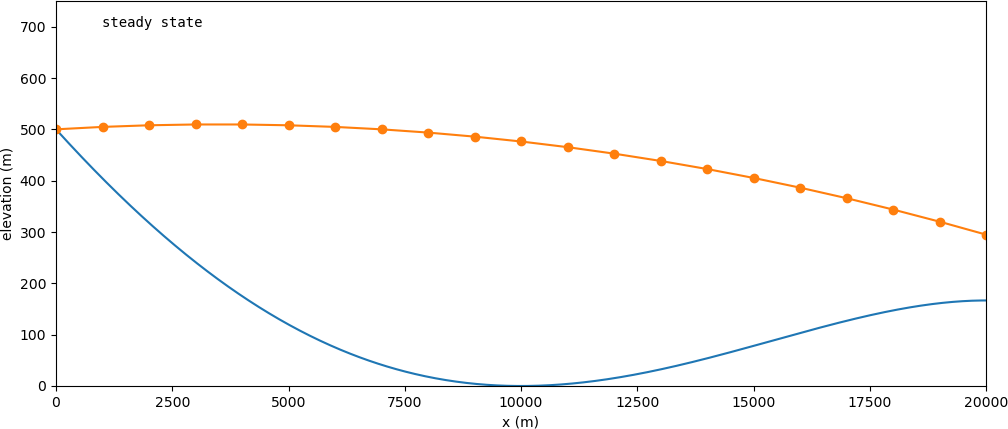
\includegraphics[width=0.7\textwidth]{steady}
\end{center}

\bigskip
\begin{itemize}
\item FIXME
\end{itemize}

\begin{block}{live demo}
\begin{itemize}
\item FIXME:
\begin{verbatim}
$ foo
\end{verbatim}
\end{itemize}
\end{block}
\end{frame}


\begin{frame}{time-dependent SKE $+$ SIA approximation}

\begin{itemize}
\item the equations of the \alert{time-dependent SIA model}, using surface elevation as the variable:
\begin{align*}
\frac{\partial s}{\partial t} + u \frac{\partial s}{\partial x} &= a + w \\
u &= - \frac{2}{n+1} A (\rho g)^n \left|\frac{\partial s}{\partial x}\right|^{n-1} \frac{\partial s}{\partial x} \left[\big(s - b\big)^{n+1} - \big(s-z\big)^{n+1}\right] \\
w &= - \int_{b}^{s} \frac{\partial u}{\partial x}(x,z)\,dz
\end{align*}
\item implementing is an exercise (exercise \textbf{13})
  \begin{itemize}
  \item[$\circ$] combine my above codes \href{https://github.com/bueler/mccarthy/blob/master/py/surace1d.py}{py/surface1d.py} and \href{https://github.com/bueler/mccarthy/blob/master/py/shallowuw.py}{py/shallowuw.py}
  \end{itemize}
\item important fact: \alert{this model \emph{diffuses} the surface elevation}
  \begin{itemize}
  \item[$\circ$] it is because ice flows downhill
  \item[$\circ$] this fact affects which time-step conditions are sufficient for stability
  \end{itemize}
\end{itemize}
\end{frame}


\begin{frame}{issues for the SIA}
\begin{itemize}
\item[] \alert{MAJOR modeling issues}
    \begin{enumerate}
    \item what do we lose when using the SIA, versus Stokes?
    \only<1>{\item how to add sliding to SIA?}
    \only<2>{\item add sliding via a \alert{membrane-stress-resolving stress balance}}
    \end{enumerate}
\item[] \alert{mathematical issues}
    \begin{enumerate}\setcounter{enumi}{2}
    \item well-posedness partially resolved \comm{let's talk separately?}
    \end{enumerate}
\item[] \alert{numerical issues}
    \begin{enumerate}\setcounter{enumi}{3}
    \item few?
    \end{enumerate}
\end{itemize}
\end{frame}


\begin{frame}{time-dependent SKE $+$ Stokes approximation}

\begin{itemize}
\item the equations of the \alert{time-dependent Glen-law Stokes model}:
\begin{align*}
\frac{\partial s}{\partial t} - \mathbf{u} \cdot \mathbf{n}_s &= a \\
\nabla \cdot \mathbf{u} &= 0 \\
-\nabla \cdot \tau_{ij} + \nabla p &= \rho\, \bm{g} \\
D\mathbf{u}_{ij} &= A \tau^{n-1} \tau_{ij}
\end{align*}
\item implementing is a major topic of current research
  \begin{itemize}
  \item[$\circ$] I do not trust \emph{anyone's} view of time stepping (yet)
  \item[$\circ$] subject (as always) to \alert{$s \ge b$}
  \end{itemize}
\item stopping here!
  \begin{itemize}
  \item[$\circ$] but projects 13, 14 look at numerical solutions of the Stokes equations (w/o SKE)
  \end{itemize}
\end{itemize}
\end{frame}


\begin{frame}{issues for any Stokes model}
\begin{itemize}
\item[] \alert{MAJOR modeling issues}
    \begin{enumerate}
    \item \alert{sliding laws} determine the basal stress state; what's good?
    \item how to adapt Stokes to compressible (e.g.~across CTS) ice?
    \end{enumerate}
\item[] \alert{mathematical issues}
    \begin{enumerate}\setcounter{enumi}{2}
    \item \dots \quad \comm{I'm happy to talk separately \dots}
    \end{enumerate}
\item[] \alert{numerical issues}
    \begin{enumerate}\setcounter{enumi}{3}
    \item as a practical matter, use a powerful finite element library
        \begin{itemize}
        \item[$\circ$] Firedrake? Elmer? FENiCs? Deal.ii? Dune? Moose? \dots
        \end{itemize}
    \item now worry about solver performance!
    \item I'm sure the issues will be fully resolved by 2100
    \end{enumerate}
\end{itemize}
\end{frame}


\begin{frame}{Summary}
FIXME
\end{frame}

\begin{frame}[standout]
  Questions?
\end{frame}


\appendix


\setbeamerfont{bibliography item}{size=\scriptsize}
\setbeamerfont{bibliography entry author}{size=\scriptsize}
\setbeamerfont{bibliography entry title}{size=\scriptsize}
\setbeamerfont{bibliography entry location}{size=\scriptsize}
\setbeamerfont{bibliography entry note}{size=\scriptsize}
\setbeamertemplate{frametitle continuation}{}  % remove the "i"

\begin{frame}[allowframebreaks]
\frametitle{References}
\setbeamertemplate{bibliography item}[text]

  \bibliography{slides}
  \bibliographystyle{alpha}
\end{frame}


\subsection[]{extra slides}


\begin{frame}[standout]
Extra Slides

\begin{itemize}
\item 1. derive SKE from mass conservation
%\item 2. something
\end{itemize}
\end{frame}

\begin{frame}{SKE from mass conservation}
\begin{center}
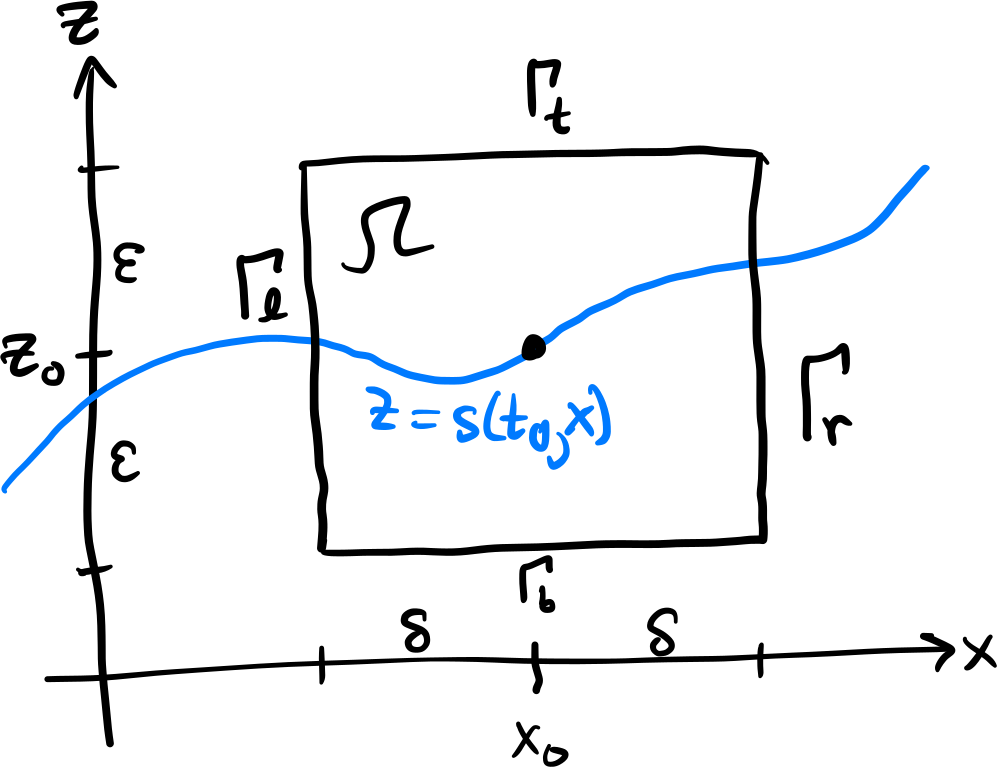
\includegraphics[width=0.65\textwidth]{skederive.png}
\end{center}

\begin{itemize}
\item these extra slides derive the surface kinematical equation (SKE) from mass conservation applied over a rectangle
\item contrast with standard (dismissive!) derivations \cite{GreveBlatter2009,SchoofHewitt2013}
\end{itemize}
\end{frame}


\begin{frame}{SKE from mass conservation 2}
\begin{center}
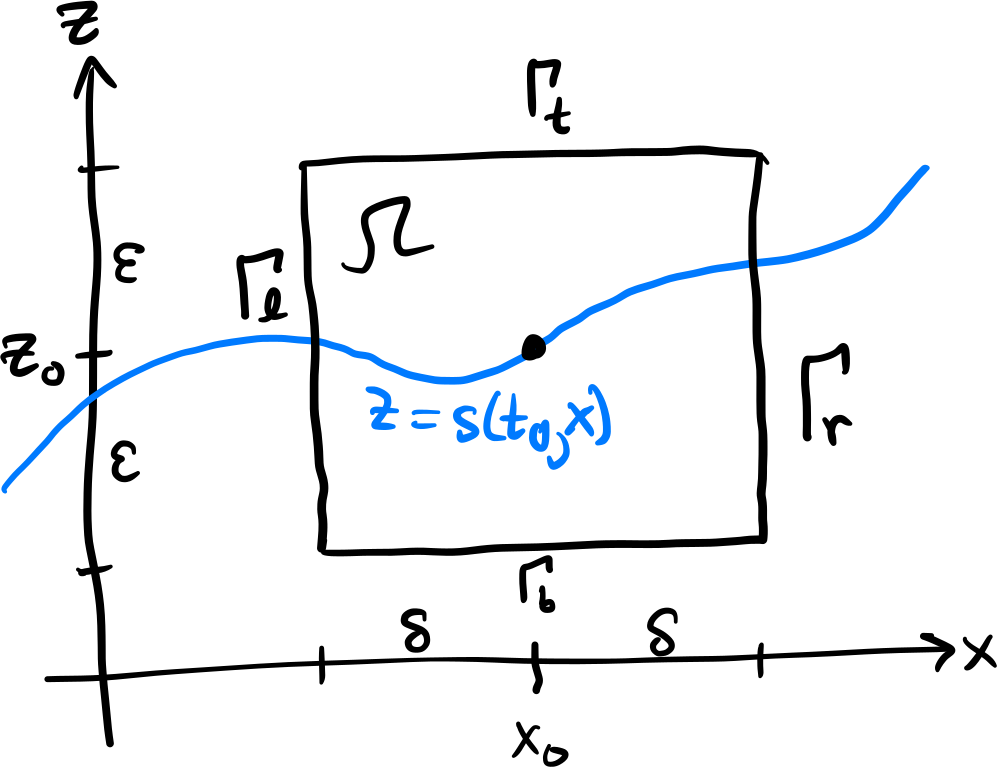
\includegraphics[width=0.4\textwidth]{skederive.png}
\end{center}

\begin{itemize}
\item $\Omega = (\text{rectangle centered at} (x_0,z_0)) =[x_0-\delta,x_0+\delta] \times [z_0-\eps,z_0+\eps]$

    \begin{itemize}
    \item[$\circ$] where $s(t_0,x_0)=z_0$
    \end{itemize}
\item let $M(t)$ be the mass of (constant-density) ice within $\Omega$ at time $t$:
   $$M(t) = \int_\Omega \rhoi \mathbb{1}_{\{z<s(t,x)\}}\,dx\,dz = \rhoi \int_{x_0-\delta}^{x_0+\delta} s(t,x) - z_0 + \eps\,dx$$
\item notation: $\bpsi =$ mass flux, $\hbn =$ outward unit normal
\end{itemize}
\end{frame}


\begin{frame}{SKE from mass conservation 3}
\begin{center}
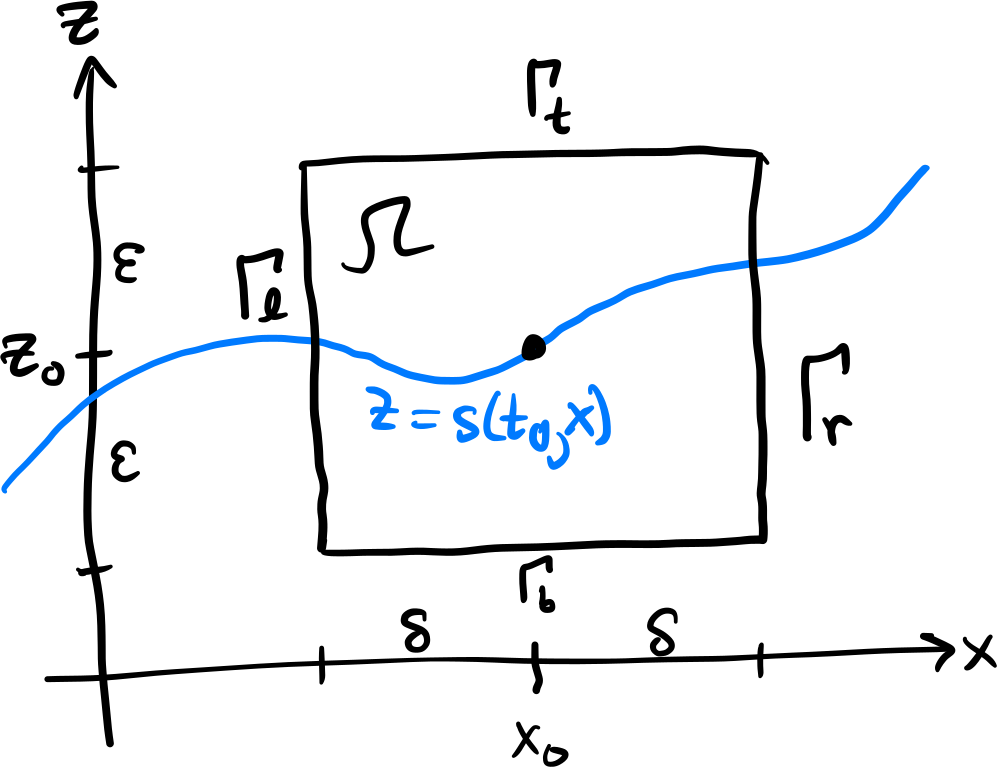
\includegraphics[width=0.4\textwidth]{skederive.png}
\end{center}

\vspace{-3mm}

\begin{itemize}
\item assumptions:
    \begin{itemize}
    \item[$\circ$] there are no mass sources within $\Omega$
    \item[$\circ$] there is an interval of time $t$ so that \,$z_0-\eps < s(t,x) < z_0 + \eps$
    %\item[$\circ$] ice has constant density $\rhoi$
    \item[$\circ$] the ice velocity $\bu(t,x,z)=(u,w)$ is defined on $\{z<s(t,x)\}$
    \item[$\circ$] the SMB $a(t,x)$ is a mass flux only across $\Gamma_t$:
        \begin{itemize}
        \item $\bpsi\big|_{\Gamma_t} = - \rho_i a(t,x) \hbz$  \comm{note $a>0$ is precipitation}
        \end{itemize}
    \item[$\circ$] the other mass fluxes are advective:
        \begin{itemize}
        \item $\bpsi\big|_{\Gamma_b} = \rho_i w(t,x,z_0-\eps) \hbz$
        \item $\bpsi\big|_{\Gamma_{\{\ell,r\}}} = \begin{cases} \rho_i u(t,x_{\{\ell,r\}},z) \hbx, & \text{if } z < s(t,x_{\{\ell,r\}}), \\ \bzero, & \text{otherwise} \end{cases}$
        \end{itemize}
    \end{itemize}
\end{itemize}
\end{frame}


\begin{frame}{SKE from mass conservation 4}

\begin{itemize}
\item mass is conserved:
\begin{align*}
\frac{dM}{dt} &= - \int_{\partial \Omega} \bpsi \cdot \hbn\,ds \\
  &= \underbrace{\rhoi \int_{x_0-\delta}^{x_0+\delta} a(t,x)\,dx}_{\Gamma_t} + \underbrace{\rhoi \int_{x_0-\delta}^{x_0+\delta} w(t,x,z_0-\eps)\,dx}_{\Gamma_b} \\
  &\quad + \underbrace{\rhoi \int_{z_0-\eps}^{s(t,x_0-\delta)} u(t,x_0-\delta,z)\,dz}_{\Gamma_\ell} - \underbrace{\rhoi \int_{z_0-\eps}^{s(t,x_0+\delta)} u(t,x_0+\delta,z)\,dz}_{\Gamma_r}
\end{align*}

\end{itemize}
\end{frame}


\begin{frame}{SKE from mass conservation 5}

\begin{itemize}
\item time derivative:
\begin{align*}
\frac{dM}{dt} &= \lim_{\omega\to 0} \frac{M(t+\omega) - M(t)}{\omega} \\
    &= \lim_{\omega\to 0} \frac{\rhoi}{\omega} \int_\Omega \mathbb{1}_{\{z<s(t+\omega,x)\}} - \mathbb{1}_{\{z<s(t,x)\}}\,dz\,dx \\
    &= \lim_{\omega\to 0} \frac{\rhoi}{\omega} \int_{x_0-\delta}^{x_0+\delta} s(t+\omega,x) - s(t,x)\,dx \\
    &= \rho_i \int_{x_0-\delta}^{x_0+\delta} \frac{\partial s}{\partial t}(t,x)\,dx
\end{align*}
\item assume smoothness sufficient for Taylor expansions on $\Omega$:
\begin{align*}
a(t,x) &= a(t,x_0) + O(\delta) \\
u(t,x,z) &= u(t,x_0,z_0) + O(\delta) + O(\eps) \\
w(t,x,z) &= w(t,x_0,z_0) + O(\delta) + O(\eps) \\
\frac{\partial s}{\partial t}(t,x) &= \frac{\partial s}{\partial t}(t,x_0) + O(\delta)
\end{align*}
\end{itemize}
\end{frame}


\begin{frame}{SKE from mass conservation 6}

\begin{itemize}
\item combine mass conservation, time derivative, and Taylor:
\begin{align*}
2\delta \rhoi \frac{\partial s}{\partial t}(t,x_0) + O(\delta^2) &= 2\delta \rhoi a(t,x_0) + O(\delta^2) \\
  &\quad + 2\delta \rhoi w(t,x_0,z_0) + O(\delta^2) + O(\delta \eps) \\
  &\quad - \rho_i u(t,x_0,z_0) \Big[s(t,x_0+\delta) - s(t,x_0-\delta)\Big] + O(\delta \eps)
\end{align*}
\item divide by $2\rhoi\delta$:
\begin{align*}
\frac{\partial s}{\partial t}(t,x_0) &= a(t,x_0) + w(t,x_0,z_0) - u(t,x_0,z_0) \frac{s(t,x_0+\delta) - s(t,x_0-\delta)}{2\delta} \\
  &\quad  + O(\delta) + O(\eps)
\end{align*}
\item limit $\delta, \eps \to 0$ to get SKE at $(t,x_0,z_0) = (t,x_0,s(t,x_0))$:
  $$\frac{\partial s}{\partial t} = a + w - u \frac{\partial s}{\partial x}$$
\end{itemize}
\end{frame}

\end{document}
